\section{Architecture of the solution}\label{sec:architecture}

The scientific part of the work is a pipeline that moves from dated data snapshots to interval forecasts, from forecasts to evaluated contrasts, and from contrasts to the figures and tables of this paper. The pipeline is shown in Figure~\ref{fig:pipeline}. Two further layers, a platform module and an explanation layer, are engineering artefacts built on the same interval method; they are described briefly in Section~\ref{sec:platform} and are labelled as such, because no scientific claim of the paper depends on them.

\begin{figure}[t]
\centering
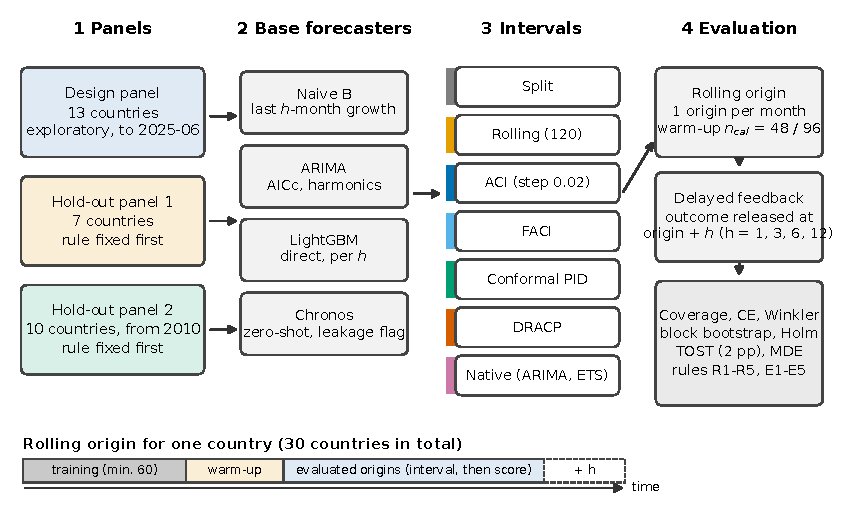
\includegraphics[width=\linewidth]{figures/fig_pipeline.pdf}
\caption{The experimental pipeline: dated and hashed data snapshots, point forecasters, interval methods, evaluation (coverage, calibration error, interval score, block bootstrap, Holm, TOST, minimum detectable difference) and the generation of the paper's figures and tables. The platform and explanation layers are engineering artefacts built on the interval method.}
\label{fig:pipeline}
\end{figure}

\subsection{Pipeline}\label{sec:pipeline}

\paragraph{Data.} Monthly IMF consumer price indices, exchange rates and the Brent crude price are downloaded by Node scripts into dated JSON snapshots whose SHA-256 hashes are recorded (Section~\ref{sec:snapshots} and Appendix~\ref{app:data}). A loader chains the snapshots on the CPI level at their last common month, cuts series into stretches of consecutive months, and labels every evaluated row by sample (exploratory, hold-out or second hold-out) from its target month and country.

\paragraph{Forecasters.} Each base forecaster (naive A and B, ETS, ARIMA, LightGBM, Chronos) is a function of the information dated at or before the forecast origin. Look-ahead is excluded by construction and by tests that corrupt all data after the origin and check that the forecast is unchanged.

\paragraph{Intervals.} The six interval methods consume the point forecast through a streaming interface (\texttt{fit}, \texttt{predict\_one}, \texttt{update\_one}) in which the outcome of the forecast made at origin $j$ is returned only at origin $j+h$ (equation~\eqref{eq:released}). The default is therefore the delayed-feedback setting; the instant-feedback diagnostic is a separate, labelled run.

\paragraph{Evaluation.} Per-row results (forecast, interval bounds, outcome, flags) are summarised into coverage, calibration error, width and interval score, and the contrasts of Section~\ref{sec:contrasts} are computed with the moving-block bootstrap, Holm correction, TOST and the power simulation of Section~\ref{sec:mde}. Robustness analyses (leave-one-country-out, other base models, feedback delay, width) use only existing intervals.

\paragraph{Assets.} The figures and tables of this paper are generated from the committed result tables by a single script, so that every number in a table or figure has a path back to a result file. Numbers quoted in the running text were written from the project's manuscript and its result documents.

\subsection{The platform and the explanation layer (engineering)}\label{sec:platform}

\paragraph{Platform module.} The repository contains a module of the application that serves calibrated inflation intervals for the 13 design economies through a FastAPI endpoint (\texttt{GET /api/v1/inflation/calibrated-forecast}), with a page of the React front end that shows the measured backtest coverage next to the nominal level. The service reads a CPI snapshot and forms the point forecast as $h$ times an exponentially weighted moving average of past monthly log growth (smoothing parameter 0.2). It issues intervals by ACI on absolute residuals over a rolling calibration window of 120 months with step 0.02, with delayed feedback, and requires at least 30 revealed residuals before issuing an interval. The point forecast, the minimum calibration size (30 against the benchmark's warm-up of 48) and the data differ from the benchmark, which uses LightGBM and other base models. The benchmark results therefore bear on the module only through the interval method, and the module's own backtest coverage is displayed to users. ACI was chosen for the module as an adaptive method that is better calibrated than a one-shot calibration and than native intervals, and that is simple to implement and explain; the benchmark did not show it to be better than a rolling window on all panels.

\paragraph{Explanation layer.} A service receives a question about a country and a horizon, calls the platform endpoint as a tool and answers in English, Russian or Kazakh. Its evaluation was specified in the eighth protocol entry before any request was made: 13 countries, 4 horizons, 3 question types and 3 languages give 468 prompts, each answered in two conditions (with the tool result in the context, and without it as an ungrounded baseline), so 936 calls. The metrics are computed by program and not by a judge model: numerical faithfulness, omission rate and coverage overstatement, with Wilson 95\% intervals, and a manual review of 30 answers per language for fluency and terminology; there is no pass threshold. After the protocol entry the harness was changed to call only an OpenAI-compatible endpoint (a LiteLLM proxy, with the model identifier taken from an environment variable); the design of the evaluation described above did not change in this respect. The service and the harness were tested with a deterministic fake client that only exercises the code.

\textbf{The evaluation of the explanation layer has not been run on a real language model, and no result is reported.} The output of the fake client is not a result. No claim of this paper depends on this component, and nothing is claimed about the faithfulness, omissions or overstatements of such a layer.
